\section{Ток смещения. Полная система уравнений Максвелла.}

\[
\begin{cases}
    \mathrm{div}\vec{D}=4\pi\rho \\
    \mathrm{rot}\vec{E}-\frac{1}{c} \frac{\partial \vec{B}}{\partial t}    
\end{cases}
\]

Для замкнутости необходимы дополнительные материальные уравнения:

Например: \( \vec{D}=\varepsilon\vec{E} \)

В интегральной форме: \( \oiint \vec{D}d\vec{S}=4\pi Q=4\pi \underset{\mathbb{V} }{\iiint}\rho dV \) 

\[
\oint\vec{E}d\vec{l}=-\frac{1}{c}\frac{d\Phi}{dt}\text{ , где } \Phi=\underset{\mathbb{S} }{\iint}\vec{B}d\vec{S}  
\]

\[
\begin{cases}
    \mathrm{div}\vec{D}=4\pi\rho \\
    \mathrm{rot}\vec{E}=-\frac{1}{c} \frac{\partial \vec{B}}{\partial t} \\
    \mathrm{div}\vec{B}=0 \\
    \mathrm{rot}\vec{B}=\frac{4\pi}{c}\vec{j}      
\end{cases}
\]

Мат. уравнения: \( \vec{B}=\mu\vec{H} \qquad \vec{D}=\varepsilon\vec{E} \)

З.С.З.: \( \frac{\partial\rho}{\partial t} +\mathrm{div}\vec{j}=0\Rightarrow \mathrm{div}\vec{j} =-\frac{\partial\rho}{\partial t}  \) 

\[
\mathrm{div}\vec{j}= \frac{c}{4\pi}\mathrm{div}\mathrm{rot}\vec{H}\equiv     0
\]

\begin{minipage}[c]{0.4\textwidth} % Левая часть: изображение
    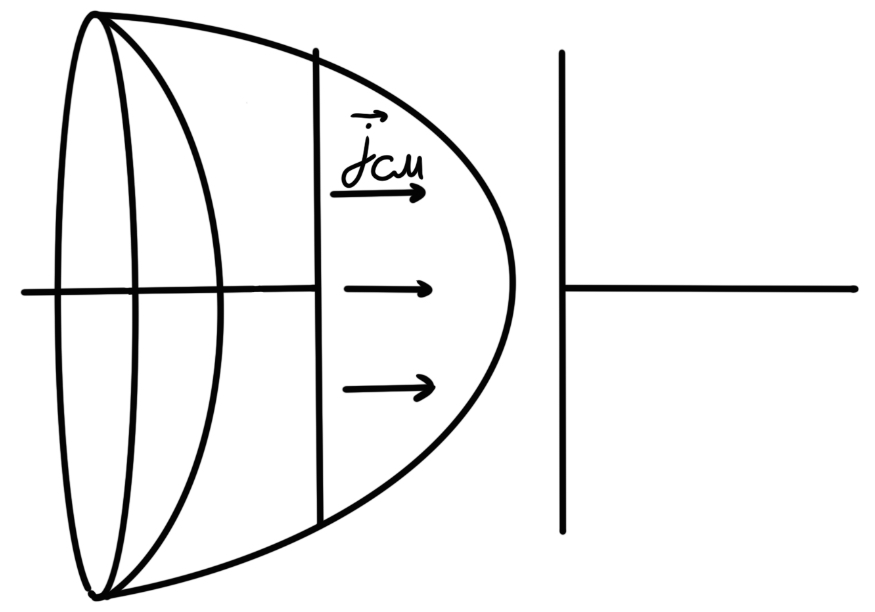
\includegraphics[width=\textwidth]{im/88.png}% Ваше изображение
\end{minipage}%
\hfill
\begin{minipage}[c]{0.6\textwidth} % Правая часть: текст
\[\underset{\delta\mathbb{S} }{\oint} \vec{H}d\vec{S}=\frac{4\pi}{c}\underset{\mathbb{S}}{\iint} \vec{j}d\vec{S} \]
\end{minipage}

\begin{minipage}[c]{0.3\textwidth} % Левая часть: изображение
    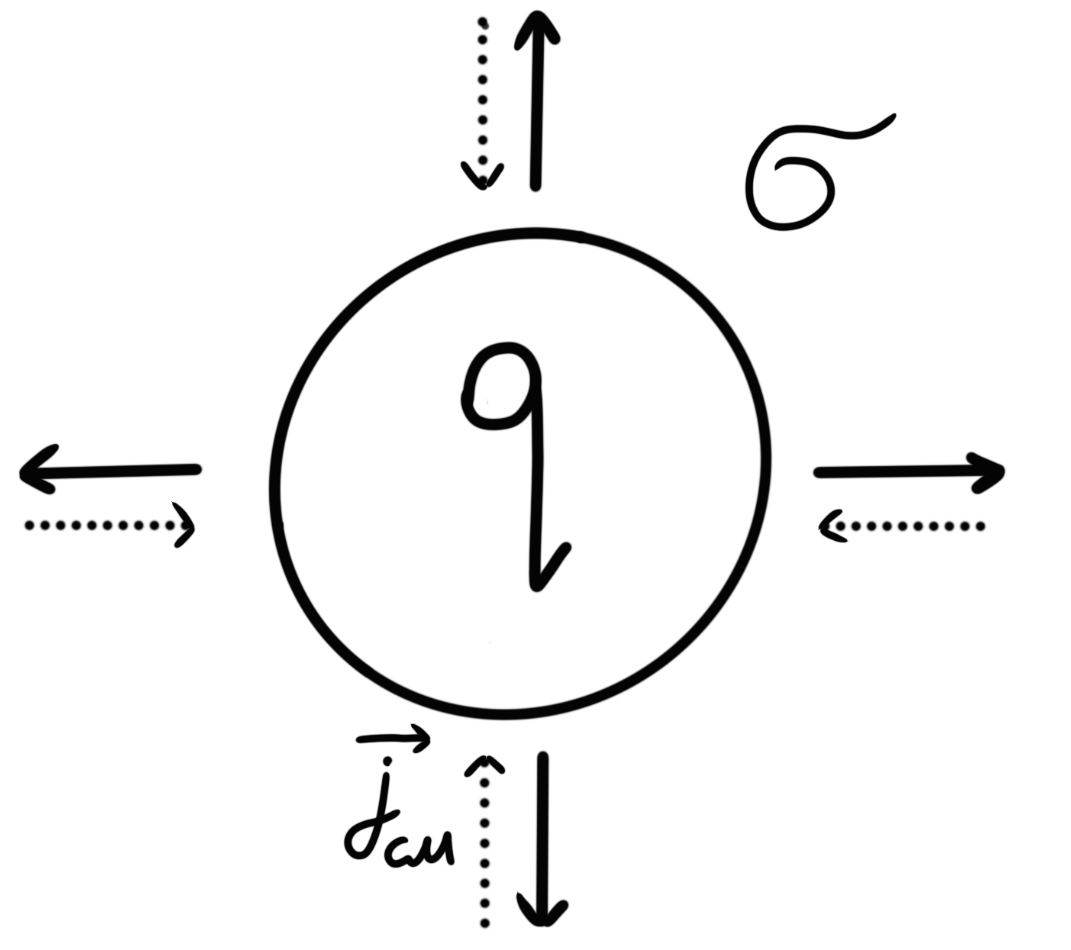
\includegraphics[width=\textwidth]{im/89.png}% Ваше изображение
\end{minipage}%
\hfill
\begin{minipage}[c]{0.6\textwidth} % Правая часть: текст
\[
\begin{aligned}
&\text{Максимальная релаксация:} \\
&\text{магнитное поле всюду ноль отсюда}:\\
&\mathrm{rot}\vec{H}=0 \text{ , отсюда } \vec{j}=0 \\
&\text{, а это не верно, значит уравнение не полное}
\end{aligned}
\]
\end{minipage}

Дополнение:

\[
\mathrm{rot}\vec{H}=\frac{4\pi}{c}\left( \vec{j}+\vec{j}_{\text{см}} \right)\Rightarrow \mathrm{div}\vec{j}=-\mathrm{div}\vec{j_{\text{см}}}=-\frac{\partial\rho}{\partial t}=-\frac{1}{4\pi}\mathrm{div} \frac{\partial \vec{D}}{\partial t}        
\]

Если принять \( \vec{j_{\text{см}}}=\frac{1}{4\pi}\frac{\partial \vec{D}}{\partial t}     \) , то получим дополненое уравнение Максвелла:

\[
\boxed{\mathrm{rot}\vec{B}=\frac{4\pi}{c}\vec{j}+\frac{1}{c} \frac{\partial\vec{D}}{\partial t}    }
\]

\begin{gather*}
    \vec{D}=\vec{E}+4\pi\vec{P} \\
    \frac{\partial \vec{D}}{\partial t}= \frac{\partial \vec{E}}{\partial t} +4\pi \frac{\partial \vec{P}}{\partial t}  
\end{gather*}

Уравнение Максвелла:

\[
\begin{aligned}
    \begin{cases}
        \mathrm{div}\vec{D}=4\pi\rho \\
        \mathrm{rot}\vec{E}=-\frac{1}{c} \frac{\partial\vec{B}}{\partial t} \\
        \mathrm{div}\vec{B}=0 \\
        \mathrm{rot}\vec{H}=\frac{4\pi}{c}\vec{j}+\frac{1}{c} \frac{\partial D}{\partial t}      
    \end{cases}
    \text{ }
    \begin{array}{ll}
        \oiint \vec{B}d\vec{S}=0 \\
        \oint\vec{H}d\vec{l}=\frac{4\pi}{c}I+\frac{1}{c} \frac{\partial}{\partial t}\iint \vec{D}d\vec{S} \\
        \text{где } I=\underset{\mathbb{S}}{\iint}\vec{j}d\vec{S} 
    \end{array}
\end{aligned}
\]

Мат. уравнения:

\[
\vec{D}=\varepsilon\vec{E} \qquad \vec{B}=\mu\vec{H}
\]

Закон сохранения зарядов уже входит в уравния Максвелла.